
%
%===================================================================================================
% Universidade: Universidade Federal de Goiás - UFG
% Curso.......: Ciência da Computação - BCC
% Disciplina..: Estruturas de Dados - 1
% Ano/Semestre: 2017/2
%
% Professor...: Wanderley de Souza Alencar
%
% Material....: Modelo de Slides para Apresentação de Seminário
%
%===================================================================================================
%
\documentclass[blue,compress]{beamer}

%\usepackage[dvips]{graphicx}            % to include images
\usepackage[english,portuguese,brazil]{babel}
%\usepackage[T1]{fontenc} 
%\usepackage[ansinew]{inputenc} 
\usepackage[utf8x]{inputenc}  
\usepackage{graphicx}
\usepackage{longtable}
\usepackage{float}
\usepackage{fancyvrb}
\usepackage{amsfonts}
\usepackage{amsmath}
\usepackage{amssymb}
\usepackage{url}
% \usepackage[vlined,titlenumbered,algo2e,ruled]{algorithm2e} 
\usepackage[english, ruled, vlined, longend]{algorithm2e}
\usepackage{indentfirst}
\usepackage{subfigure}
%\usepackage{times}

\usepackage{listings}
\definecolor{listinggray}{gray}{0.9}
\definecolor{lbcolor}{rgb}{0.9,0.9,0.9}
\lstset{
    language=c,
    basicstyle=\scriptsize,
    upquote=true,
    aboveskip={0.1\baselineskip},
    columns=fullflexible,
    showstringspaces=false,
    numbers=left,
    numberstyle=\tiny\color{gray},
    stepnumber=1,
    numbersep=5pt, 
    extendedchars=true,
    breaklines=true,
    showtabs=false,
    showspaces=false,
    identifierstyle=\ttfamily,
    keywordstyle=\color[rgb]{0,0,1},
    %commentstyl-e=\color[rgb]{0.133,0.545,0.133},
    stringstyle=\color[rgb]{0.627,0.126,0.941},
    tabsize=3,
}


\usetheme{Warsaw}
\usefonttheme{professionalfonts}
\usenavigationsymbolstemplate{}
\title{Árvore 2-3}


\author[Estudantes]{ Luigi Wagner \\ Rafael Alessandro \\ Rafael Falcão
}
\institute{
    Curso de Ciência da Computação -- Disciplina: Estruturas de Dados -- 1 \\
	Instituto de Informáica \\
	Universidade Federal de Goiás
}

\date{\today}

\AtBeginSection[]
{
 \begin{frame}<beamer>
  \frametitle{Sumário}
  \tableofcontents[currentsection]
 \end{frame}
}


\begin{document}
\frame{\titlepage}
%
%---------------------------------------------------------------------------------------------------
% Primeiro Tópico
%---------------------------------------------------------------------------------------------------
%
\section[\thesection]{Introdução}

\frame { \frametitle{Introdução}
    Uma Árvore 2-3 é uma árvore onde cada nó com filho (nó interno) tem também 2 filhos (2-node) e 1 elemento de dados (chave) ou 3 filhos (3-nodes) e 2 elementos de dados (chaves).
Os nós externos a árvore (nós-folha) não tem filhos e possuem um ou dois elementos de dados (chaves).
}

%\frame { \frametitle{Introdução}
%	Cada \texttt{seção} (ou \emph{section}, em LaTeX) deve corresponder a um dos tópicos a serem abordados naquele tema.
%	\newline
%	\newline
%	As \texttt{seções} podem, livremente, serem subdividas em subseções e subsubseções.
%}

\frame { \frametitle{Introdução}
	\begin{block}{Propriedades}
		As principais \texttt{propriedades} de uma Árvore 2-3 são:
		%\newline
		\newline
		\begin{itemize}
		      \item Cada nó interno tem dois filhos (2-node) se tem uma chave, ou três filhos (3-node) se tem duas chaves; 
		      \item Cada nó não-folha tem 2 ou 3 filhos. Se tem 2 filhos tem 1 item de dados e se tem 3 filhos tem 2 itens de dados;
		      \item Todos os dados são ordenados;
		      \item Todas as folhas estão no mesmo nível;
		      \item Cada nó folha tem 1 ou 2 campos.
		      %\item $\dots$
		\end{itemize}
        Como, por exemplo:
	\end{block}
}

\frame { \frametitle{Introdução}
	\begin{block}{\textit{Teorema de Kleene}}
		Para uma dada linguagem $\mathcal{L}$, são equivalentes as afirmações:
		\begin{enumerate}
		      \item $\mathcal{L}$ é reconhecida por um autômato determinístico;
		      \item $\mathcal{L}$ é reconhecida por um autômato não determinístico;
		      \item $\mathcal{L}$ é descrita por uma expressão regular.
		\end{enumerate}
	\end{block}
}

\frame { \frametitle{Introdução}
	\begin{block}{Bloco}
		Um \texttt{bloco} pode conter figuras, tabelas, listas, etc.
	\end{block}
}
%
%---------------------------------------------------------------------------------------------------
% Segundo Tópico
%---------------------------------------------------------------------------------------------------
%
\section[\thesection]{}

\frame { \frametitle{Segundo Tópico}
	Aqui começamos um segundo tópico, ou seja, a segunda seção dos \emph{slides}
	\begin{itemize}
	 	\item Operações sobre linguagens;
	 	\item Expressões regulares.
	\end{itemize}
}

\frame { \frametitle{Segundo Tópico}
	\begin{block}{Continuando}
  		Como antes, o tópico pode ser um \texttt{bloco}...	
    \end{block}
}

\frame { \frametitle{Segundo Tópico}	
    O tópico pode ter uma figura:
	\begin{figure}[htbp]
		\centering
		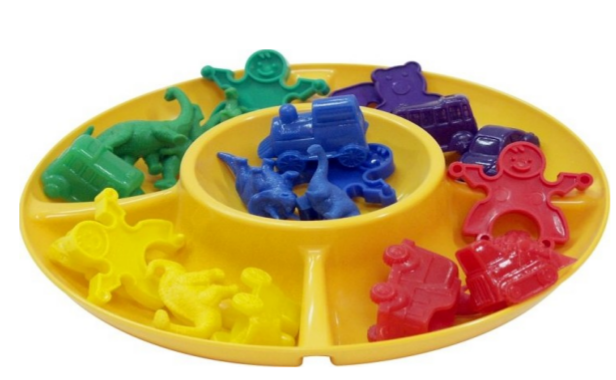
\includegraphics[width=0.8\textwidth]{./fig/classificador01.png}	
    \end{figure}
}

\frame { \frametitle{Segundo Tópico}
    Pode fazer uma pergunta usando uma figura?
	\begin{figure}[htbp]
		\centering
		
\includegraphics[width=0.50\textwidth]{./fig/perguntador01.png}	
    \end{figure}
}

\frame { \frametitle{Segundo Tópico}
	\begin{block}{Matemático}
		Um \emph{slide} pode utilizar símbolos matemáticos, como:
		\begin{itemize}
    		\item $\epsilon$ é uma letra grega que normalmente denota quantidades extremamente pequenas; 
    		\item $\alpha$, $\beta$, e $\gamma$ são outras letras gregas.
   		\end{itemize}
	\end{block}
}

\frame { \frametitle{Segundo Tópico}
	\begin{block}{Programas}
		Se precisar utilizar \texttt{algoritmos} ou \texttt{programas} em seus \emph{slides}, utilize-os da maneira 
mostrada a seguir...
		\begin{itemize}
		      \item embutido dentro do comando \texttt{lstlisting};
		      \item colocado num arquivo separado e utilizando o comando \texttt{lstinputlisting}.
		\end{itemize}

	\end{block}
}

\begin{frame}[fragile] \frametitle{Segundo Tópico}
  \vspace{-0.3cm}
  \begin{block}{Programa 01}
     	\begin{lstlisting}
int main (void) 
{
  	char *ponteiro; 
  	
  	ponteiro = malloc(1);
  	if (ponteiro != NULL) { 
    		printf("Informe um caracter: ");
    		scanf("%c", ponteiro);
  	}
  	return(EXIT_SUCCESS);
}     
    	\end{lstlisting}
  \end{block}
\end{frame}

\begin{frame}{Segundo Tópico}
	\begin{block}{Programa 02}
		\lstinputlisting[language=c]{./programas/declaracaoEstruturas.c}
  	\end{block}      
\end{frame}
%
%---------------------------------------------------------------------------------------------------
% Terceiro tópico
%---------------------------------------------------------------------------------------------------
%
\section[\thesection]{Terceiro Tópico}

\frame { \frametitle{Terceiro Tópico}
	\begin{block}{Tabelas}
		Qualquer recursos disponível no \texttt{LaTeX} e seus pacotes complementares podem ser utilizados, desde que ao 
final a equipe gere um arquivo compactado (extensão .zip) contendo toda a ``\emph{pasta}'' com os \emph{slides} 
desenvolvidos.
		\newline
		\newline
		A pasta gerada também deverá conter um arquivo \texttt{.pdf} com os \emph{slides} utilizados.
	\end{block}
}

\frame { \frametitle{Terceiro Tópico}
	\begin{block}{Exemplo 01}
		Exemplos devem utilizar um \texttt{bloco} para serem apresentados, como o que está acontecendo neste momento, 
ou seja, um bloco está sendo utilizado e seu título é \texttt{Exemplo 01}. 
		\newline
		\newline 
		Você também pode utilizar \textcolor{blue}{cores} para dar destaque no texto.
	\end{block}
}
%
%---------------------------------------------------------------------------------------------------
% Questionário
%---------------------------------------------------------------------------------------------------
%
\section[\thesection]{Questionário}

\frame { \frametitle{Questionário}
	Deve haver, ao final, uma seção dedicada à apresentação de um questionário com pelo menos $05$ (cinco) questões, e 
suas respectivas respostas esperadas.
	\newline
	\newline
	Cada questão deverá ser um \texttt{bloco}, o mesmo ocorrendo com a resposta esperada.
	\newline
	\newline
	Veja o exemplo....
}

\frame { \frametitle{Questionário}
	\begin{block}{Questão 01}
	      Enunciado da primeira questão, se necessário com figuras, tabelas, e tudo mais.
	\end{block}
}	

\frame { \frametitle{Questionário}
	\begin{block}{Questão 01 -- Resposta Esperada}
	      Bloco com a resposta esperada para a primeira questão.
	\end{block}
}	
%
%---------------------------------------------------------------------------------------------------
% Referências Bibliográficas
%---------------------------------------------------------------------------------------------------
%
\section[\thesection]{Referências Bibliográficas}

%\frame { \frametitle{Referências Bibliográficas}
%	A última seção dos \emph{slides} deve apresentar as referências bibliográficas do trabalho: artigos, 
%\emph{websites}, livros, capítulos de livros, etc.
%	\newline
%	\newline
%	Veja o exemplo...
%}


\frame { \frametitle{Referências Bibliográficas}
	\begin{itemize}
	 \item \url{https://pt.wikipedia.org/wiki/\%C3\%81rvore_2-3}
	 \item COOPER, K. and TORCZON, L. -- 2011 : \textit{Chapter 2 -- Scanners};
	 \item GRUNE, \textit{et al.} -- 2012 : \textit{Chapter 2 -- Program Text to Tokens -- 
Lexical Analysis}.
	\end{itemize}
}

\frame { \frametitle{Referências Bibliográficas}
	Se desejar, pode encerrar com uma imagem, uma citação, etc.
	\begin{figure}[htbp]
		\centering
		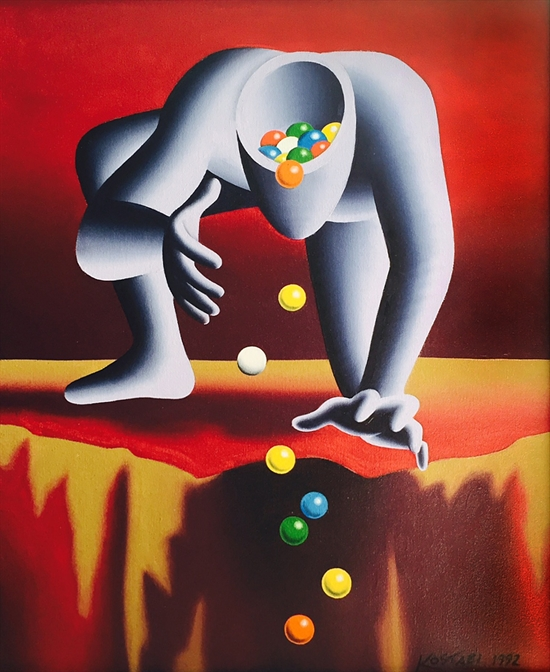
\includegraphics[width=0.50\textwidth]{./fig/MarkKostabi01.jpg}
		\caption{by Mark Kostabi.} 
\label{fig:traducaoRIparaLO}
   	\end{figure}
}

\end{document}
